\documentclass[a4paper]{article}
\usepackage{geometry}
\usepackage{graphicx}
\usepackage{natbib}
\usepackage{amsmath}
\usepackage{amssymb}
\usepackage{amsthm}
\usepackage{paralist}
\usepackage{epstopdf}
\usepackage{tabularx}
\usepackage{longtable}
\usepackage{multirow}
\usepackage{multicol}
\usepackage[hidelinks]{hyperref}
\usepackage{fancyvrb}
\usepackage{algorithm}
\usepackage{algorithmic}
\usepackage{float}
\usepackage{paralist}
\usepackage[svgname]{xcolor}
\usepackage{enumerate}
\usepackage{array}
\usepackage{times}
\usepackage{url}
\usepackage{fancyhdr}
\usepackage{comment}
\usepackage{environ}
\usepackage{times}
\usepackage{textcomp}
\usepackage{caption}
\usepackage{bbm}
\usepackage{enumitem}


\urlstyle{rm}

\setlength\parindent{0pt} % Removes all indentation from paragraphs
\theoremstyle{definition}
\newtheorem{definition}{Definition}[]
\newtheorem{conjecture}{Conjecture}[]
\newtheorem{example}{Example}[]
\newtheorem{theorem}{Theorem}[]
\newtheorem{lemma}{Lemma}
\newtheorem{proposition}{Proposition}
\newtheorem{corollary}{Corollary}

\floatname{algorithm}{Procedure}
\renewcommand{\algorithmicrequire}{\textbf{Input:}}
\renewcommand{\algorithmicensure}{\textbf{Output:}}
\newcommand{\abs}[1]{\lvert#1\rvert}
\newcommand{\norm}[1]{\lVert#1\rVert}
\newcommand{\RR}{\mathbb{R}}
\newcommand{\CC}{\mathbb{C}}
\newcommand{\Nat}{\mathbb{N}}
\newcommand{\br}[1]{\{#1\}}
\DeclareMathOperator*{\argmin}{arg\,min}
\DeclareMathOperator*{\argmax}{arg\,max}
\renewcommand{\qedsymbol}{$\blacksquare$}

\definecolor{dkgreen}{rgb}{0,0.6,0}
\definecolor{gray}{rgb}{0.5,0.5,0.5}
\definecolor{mauve}{rgb}{0.58,0,0.82}

\newcommand{\Var}{\mathrm{Var}}
\newcommand{\Cov}{\mathrm{Cov}}

\newcommand{\vc}[1]{\boldsymbol{#1}}
\newcommand{\xv}{\vc{x}}
\newcommand{\Sigmav}{\vc{\Sigma}}
\newcommand{\alphav}{\vc{\alpha}}
\newcommand{\muv}{\vc{\mu}}

\newcommand{\red}[1]{\textcolor{red}{#1}}

\def\x{\mathbf x}
\def\y{\mathbf y}
\def\w{\mathbf w}
\def\v{\mathbf v}
\def\E{\mathbb E}
\def\V{\mathbb V}
\def\ind{\mathbbm 1}

% TO SHOW SOLUTIONS, include following (else comment out):
\newenvironment{soln}{
    \leavevmode\color{blue}\ignorespaces
}{}


\hypersetup{
%    colorlinks,
    linkcolor={red!50!black},
    citecolor={blue!50!black},
    urlcolor={blue!80!black}
}

\geometry{
  top=1in,            % <-- you want to adjust this
  inner=1in,
  outer=1in,
  bottom=1in,
  headheight=3em,       % <-- and this
  headsep=2em,          % <-- and this
  footskip=3em,
}


\pagestyle{fancyplain}
\lhead{\fancyplain{}{Homework 4}}
\rhead{\fancyplain{}{CS 760 Machine Learning}}
\cfoot{\thepage}

\title{\textsc{Homework 4}} % Title

%%% NOTE:  Replace 'NAME HERE' etc., and delete any "\red{}" wrappers (so it won't show up as red)

\author{
\red{GURUPRASAD VISWANATHAN RAMESH} \\
\red{viswanathanr@wisc.edu;9082378762}\\
} 

\date{}

\begin{document}

\maketitle 


\textbf{Instructions:} Use this latex file as a template to develop your homework. Submit your homework on time as a single pdf file to Canvas. Late submissions may not be accepted. Please wrap your code and upload it to a public GitHub repo, then attach the link below the instructions so that we can access it. You can choose any programming language (i.e. python, R, or MATLAB). Please check Piazza for updates about the homework.

\red{CODE in ipynb folder: https://github.com/Guruprasad68/CS760-Machine-Learrning-Spring2023/tree/main/hw\%204}
\section{Best Prediction}
\subsection{Under 0-1 Loss (10 pts)}
Suppose the world generates a single observation $x \sim \mbox{multinomial}(\theta)$, where the parameter vector $\theta=(\theta_1, \ldots, \theta_k)$ with $\theta_i\ge 0$ and $\sum_{i=1}^k \theta_i=1$.  Note $x \in \{1, \ldots, k\}$.
You know $\theta$ and want to predict $x$. 
Call your prediction $\hat x$.  What is your expected 0-1 loss: 
$$\E[\ind_{\hat x \neq x}]$$
using the following two prediction strategies respectively?  Prove your answer.
\begin{enumerate}
    \item Strategy 1: $\hat x \in \argmax_x \theta_x$, the outcome with the highest probability.\\
    \begin{soln}
    $\E[\ind_{\hat x \neq x}]=1.P (\hat x \neq x)\ + 0.P(\hat x=x)=P(\hat x \neq x)=1-P(\hat x=x)=1 -\sum_{i=1}^k P(x=i)P(\hat x=i)= 1 - \sum_{i=1}^k \theta_i*(1/k)= 1 - \sum_{i=1}^k \theta_i/k$
    \end{soln}
    

    \item Strategy 2: You mimic the world by generating a prediction $\hat x \sim \mbox{multinomial}(\theta)$.  (Hint: your randomness and the world's randomness are independent)
    \begin{soln}
       $$\E[\ind_{\hat x \neq x}] = 1 - \sum_{i=1}^k P(\hat x =i)P(x=i) = 1 - \sum_{i=1}^k \theta_i^2$$ 
    \end{soln}
\end{enumerate}
\subsection{Under Different Misclassification Losses (6 pts)}
Like in the previous question, the world generates a single observation $x \sim \mbox{multinomial}(\theta)$. Let $c_{ij} \ge 0$ denote the loss you incur, if $x=i$ but you predict $\hat x=j$, for $i,j \in \{1, \ldots, k\}$.
$c_{ii}=0$ for all $i$. This is a way to generalize different costs of false positives vs false negatives from binary classification to multi-class classification. You want to minimize your expected loss:
$$\E[c_{x \hat x}].$$
Derive your optimal prediction $\hat x$.\\
\begin{soln}
$\E[c_{x \hat x}]=\sum_{i=1,j=1,i\neq j}^{k} P(x=i)P(\hat{x}=j)*c_{ij}=\sum_{i=1,j=1,i\neq j}^{k} c_{ij}\theta_i*\theta_j$. 

To minimize the above loss, $\sum_{i=1,i\neq j}^k \theta_i*c_{ij}=0$ for all j in [1,k].
    
\end{soln}
\section{Language Identification with Naive Bayes (8 pts each)}
Implement a character-based Naive Bayes classifier that classifies a document as English, Spanish, or Japanese - all written with 26 lower-case characters and space.

The dataset is languageID.tgz, unpack it. This dataset consists of 60 documents in English, Spanish, and Japanese. The correct class label is the first character of the filename: $y \in \{e, j, s\}$. (Note: here each file is a document in the corresponding language, and it is regarded as one data.)

We will be using a character-based multinomial Naïve Bayes model. You need to view each document as a bag of characters, including space. We have made sure that there are only 27 different types of printable characters (a to z, and space) -- there may be additional control characters such as new-line, please ignore those. Your vocabulary will be these 27 character types. (Note: not word types!)

In the following questions, you may use the additive smoothing technique to smooth categorical data, in case the estimated probability is zero. Given $N$ data samples $\{\vc{x}^{(i)}, y^{(i)}\}_{i = 1}^{N}$, where $\vc{x}^{(i)} = [x_1^{(i)}, \dots, x_j^{(i)}, \dots, x_{M_i}^{(i)}]$ is a bag of characters, $M_i$ is the total number of characters in $\vc{x}^{(i)}$, $x_{j}^{(i)} \in S, y^{(i)} \in L$ and we have $|S| = K_S, |L| = K_L$. Here $S$ is the set of all character types, and $L$ is the set of all classes of data labels. Then by the additive smoothing with parameter $\alpha$, we can estimate the conditional probability as 
$$
P_{\alpha}(a_s \mid y = c_k) = \frac{(\sum_{i = 1}^{N}\sum_{j = 1}^{M_i}\ind [x_{j}^{(i)} = a_s, y^{(i)} = c_k]) + \alpha}{(\sum_{b_s \in S}\sum_{i = 1}^{N}\sum_{j = 1}^{M_i}\ind [x_{j}^{(i)} = b_s, y^{(i)} = c_k]) + K_S \alpha},
$$
where $a_s \in S, c_k \in L$. Similarly, we can estimate the prior probability
$$
P_{\alpha}(Y = c_k) = \frac{(\sum_{i = 1}^{N}\ind [y^{(i)} = c_k]) + \alpha}{N + K_L \alpha},
$$
where $c_k \in L$ and $N$ is the number of training samples.
\begin{enumerate}
\item
Use files 0.txt to 9.txt in each language as the training data.
Estimate the prior probabilities 
$\hat p(y=e)$,
$\hat p(y=j)$,
$\hat p(y=s)$
using additive smoothing with parameter $\frac{1}{2}$. 
Give the formula for additive smoothing with parameter $\frac{1}{2}$ in this case. 
Print the prior probabilities.\\
\begin{soln}
The formula for the prior probabilities with additive smoothing is \\
$\hat p(y=c_k)=\frac{N_L + \alpha}{N+K_L\alpha}$, where $N_L$ is the number of files belonging to a particular language. The number of files in the training data, $N$ is 30, as each language contains 10 files. Therefore, \\ 
$\hat p(y=e)=\hat p(y=j)=\hat p(y=s)=\frac{10+0.5}{30+1.5}=1/3=0.33$
    
\end{soln}
\item
Using the same training data, estimate the class conditional probability (multinomial parameter) for English
$$\theta_{i,e} := \hat p(c_i \mid y=e)$$ 
where $c_i$ is the $i$-th character. That is, $c_1 = a, \ldots, c_{26} = z, c_{27} = space$.
Again, use additive smoothing with parameter $\frac{1}{2}$.
Give the formula for additive smoothing with parameter $\frac{1}{2}$ in this case. 
Print $\theta_e$ which is a vector with 27 elements.\\
\begin{soln}
    The class conditional probability for a particular character is given by the formula: 
    $\theta_{i,l_k}=\frac{N_il+\alpha}{N_{ltotal} + 27\alpha}$, where $N_il$ is the number of times $c_i$ appears in the docs of language $l$, and the $N_{ltotal}$ is the number of characters in the documents of each language.\\
    Using the above formula(coded in Python, can be found in GitHub repo):\\
    $\theta_e= [0.06015,0.01113,0.0215,0.02197,0.1053,0.01892,\\   0.01747,0.0472,0.0554,0.00142,0.003733,0.02898,0.02051,0.05792,\\
    0.06445, 0.01675,0.0005617,0.0538,0.06616,0.0801,0.02666,\\
    0.009285, 0.015495,0.001156,0.01384,0.0006275,0.1792]$
\end{soln}
\item
Print $\theta_j, \theta_s$, the class conditional probabilities for Japanese and Spanish.\\
\begin{soln}
    Using the same formula(executed in code):\\
    $\theta_j=[0.1318   , 0.010864 , 0.005486 , 0.01723  , 0.06018  , 0.003878 ,\\
       0.01401  , 0.03177  , 0.097    , 0.00234  , 0.0574   , 0.001432 ,\\
       0.0398   , 0.0567   , 0.0911   , 0.0008736, 0.0001048, 0.0428   ,\\
       0.04218  , 0.05698  , 0.0706   , 0.0002446, 0.01974  , 0.0000349,\\
       0.01415  , 0.00772  , 0.1234   ]$\\

    $\theta_s=[0.1046   , 0.00823  , 0.03754  , 0.03973  , 0.11383  , 0.008606 ,\\
       0.007183 , 0.00453  , 0.04987  , 0.00663  , 0.0002775, 0.05295  ,\\
       0.0258   , 0.05417  , 0.0725   , 0.02426  , 0.00768  , 0.0593   ,\\
       0.06573  , 0.0356   , 0.0337   , 0.00589  , 0.0000925, 0.002497 ,\\
       0.007866 , 0.002682 , 0.1682   ]$
\end{soln}
\item
Treat e10.txt as a test document $x$.
Represent $x$ as a bag-of-words count vector (Hint: the vocabulary has size 27).
Print the bag-of-words vector $x$.\\
\begin{soln}
    The count vector for e10.txt is :\\$x=[164,  32,  53,  57, 311,  55, 51, 140, 140,   3,   6,  85,  64,\\
        139, 182,  53,   3, 141, 186, 225,  65,  31,  47,   4, 38,   2,
        498]$.
\end{soln}
\item
For the $x$ of e10.txt, compute $\hat p(x \mid y)$ for $y=e, j, s$ under the multinomial model assumption, respectively.
Use the formula
$$\hat p(x \mid y) = \prod_{i=1}^d (\theta_{i, y})^{x_i}$$
where $x=(x_1, \ldots, x_d)$.
Show the three values: $\hat p(x \mid y=e), \hat p(x \mid y=j), \hat p(x \mid y=s)$.

Hint: you may notice that we omitted the multinomial coefficient.  This is ok for classification because it is a constant w.r.t. $y$. Also, Store all probabilities here and below in $\log()$ internally to avoid underflow. This also means you need to do arithmetic in log space.\\ 
\begin{soln}
    In logarithmic space, the formula becomes:
    $$\log \hat p(x \mid y) = \sum_{i=1}^d x_i\log \theta_{i,y} $$
    By raising the result of the log space likelihood estimate to $e$, we can get the value in normal space(it will be negligible as the log-likelihood will be a large negative value).\\
    The likelihood estimate in the log space for english is:-7841.865448746583.\\
The likelihood estimate in the log space for japanese is:-8771.43306428609.\\
The likelihood estimate in the log space for spanish is:-8467.282069010776.\\
(Coded the calculation, which can be found in the ipython files attached in the GitHub repo)
    
\end{soln}
\item
For the $x$ of e10.txt, use the Bayes rule and your estimated prior and likelihood, compute the posterior $\hat p(y \mid x)$.
Show the three values: $\hat p(y=e \mid x), \hat p(y=j \mid x), \hat p(y=s \mid x)$.
Show the predicted class label of $x$.\\
\begin{soln}
    Keeping the calculations in the log space, the posteriors can be estimated by adding $\log 1/3$(the prior in log space) to the estimated likelihoods in the previous question. \\
    The posterior estimate in the log space for english is:-7842.964061035251.\\
The posterior estimate in the log space for japanese is:-8772.531676574758.\\
The posterior estimate in the log space for spanish is:-8468.380681299444.
The predicted class is English as it has the largest likelihood value in the log space(raising the values to $e$ will also lead to the prediction of the document being English).
\end{soln}
\item
Evaluate the performance of your classifier on the test set (files 10.txt to 19.txt in three languages).
Present the performance using a confusion matrix. A confusion matrix summarizes the types of errors your classifier makes, as shown in the table below.   The columns are the true language a document is in, and the rows are the classified outcome of that document.  The cells are the number of test documents in that situation.  For example, the cell with row = English and column = Spanish contains the number of test documents that are really Spanish but misclassified as English by your classifier.


\begin{soln}
    The accuracy of the classifier turned out to be 100\% as all predictions turned out to be accurate. The confusion matrix for the test set is as follows:\\
    \begin{center}
\begin{tabular}{c|ccc}
& English & Spanish & Japanese \\
\hline
English & 10 & 0 & 0\\
Spanish & 0 & 10 & 0\\
Japanese& 0 & 0 & 10
\end{tabular}
\end{center}
\end{soln}
\item Take a test document.   Arbitrarily shuffle the order of its characters so that the words (and spaces) are scrambled beyond human recognition.  How does this shuffling affect your Naive Bayes classifier's prediction on this document?  Explain the key mathematical step in the Naive Bayes model that justifies your answer.\\
\begin{soln}
    I retook e10 for this task, shuffled the bag of characters of e10 randomly, and ended up with this list: ['n', 'o', 'r', 's', ' ', ' ', 'a', 'n', ' ', 'e', ' ', 'h', 'n', ' ', 'n', 'a', 'v', 'i', 'c', 'a', ...]. We can see that the order of characters doesn't make any linguistic sense. However, the count vector is again the same as the original e10s. This is because, irrespective of the order of the characters, the number of times it appears in the document doesn't change. Same count vector for the shuffled version: $[164, 32, 53, 57, 311., ...]$. Thus, the prediction of the classifier doesn't change. This can be explained due to the following reason:\\
    While we estimate the likelihood for the document, we raise the conditional probabilities of the characters to the power of the number of times it appears in the document, due to which our likelihood estimate remains the same irrespective of the order of the characters. This is due to the key property of Naive Bayes, where we consider the features involved to be independent.
\end{soln}
\end{enumerate}

\section{Simple Feed-Forward Network (20pts)}
In this exercise, you will derive, implement back-propagation for a simple neural network and compare your output with some standard library’s output. Consider the following 3-layer neural network.

\[
\hat{y} = f(x) = g(W_3\sigma(W_2\sigma(W_1x)))
\]

Suppose $x \in \mathbb{R}^d$, $W_1 \in \mathbb{R}^{d_1 \times d}$, $W_2 \in \mathbb{R}^{d_2 \times d_1}$, $W_3 \in \mathbb{R}^{k \times d_2}$ i.e. $f: \mathbb{R}^d \rightarrow \mathbb{R}^k$, Let $\sigma(z) = [\sigma(z_1), ..., \sigma(z_n)]$ for any $z \in \mathbb{R}^n$ where $\sigma(z) = \frac{1}{1 + e^{-z}}$ is the sigmoid (logistic) activation function and $g(z_i) = \frac{exp(z_i)}{\sum_{i=1}^k exp(z_i)}$ is the softmax function. Suppose the true pair is $(x, y)$ where $y \in \{0, 1\}^k$ with exactly one of the entries equal to 1, and you are working with the cross-entropy loss function given below,

\[
L(x, y) = -\sum_{i=1}^k y_i \text{log}(\hat{y}_i)
\]

\begin{enumerate}
    \item Derive backpropagation updates for the above neural network. (5 pts) \\
    \begin{soln}
        Let $W_iA_{i-1}=Z_i, X=A_0, act(Z_i)=A_i$, where $act$ is sigmoid or softmax activation depending on the layer. Therefore, $\hat{y}=g(Z_3)=A_3$ . For the gradient update step, we are mainly looking at the derivatives of the loss function, $L(x, y) = -\sum_{i=1}^k y_i \text{log}(\hat{y}_i)$ with respect to the weights of the layers $W_i$, and the other derivative terms are going to help us arrive at these main derivatives. Hereafter, I will be referring to the derivatives of the loss only in terms of the vector, i.e., $\frac{dL}{dX}$ will be referred to as dX.\\

        \begin{enumerate}
            \item First, let us work on the derivative $dW_3$. Using chain rule, it is: $dW_3=dA_3\frac{dA_3}{dZ_3}\frac{dZ_3}{dW_3}$. Let us first compute $\frac{dA_3}{dZ_3}$. 

        $A_3=[a_1,a_2,a_3,...,a_k]$. Similarly, $Z_3=[z_1,z_2,...,z_k]$. And since the activation is softmax, in this case, we can write $a_i=\frac{\exp{z_i}}{\sum \exp{z_j}}$. Thus, for calculating the jacobian for $A_3$ w.r.t $Z_3$, we need to look at two cases, the diagonal elements of the jacobian and the off-diagonal elements. The first can be represented as $\frac{da_i}{dz_i}$, and second will be $\frac{da_i}{dz_j}$.

        Calculating derivative $\frac{da_i}{dz_i}$:
        $a_i$ can be written as $\frac{\exp{z_i}}{\exp{z_i}+\sum_{l \neq i} \exp{z_l}}$ and the derivative is $a_i(1-a_i)$. 
        Similarly, the derivative for  $\frac{da_i}{dz_j}$ is $-a_ia_j$.

        Now, we have $\frac{da_i}{dz_j}$. The next step is to plug in with $da_j$.\\

        $dA_3=-\sum_{i=1}^k y_i/a_i$ and $dZ_3/dW_3=A_2$.\\

        Substituting these terms in the chain rule expansion of $dW_3$, we get $dW_3=dZ_3A_2^T=(A_3-Y_3)A_2^T$.

        \item Next is to get $dW_2$, for which $dZ_2$ is required. \\
        $dZ_2=dZ_3*\frac{dZ_3}{dA_2}*\frac{dA_2}{dZ_2}=W_3^T(A_3-Y_3)*(\sigma(Z_2)(1-\sigma(Z_2)))$.\\
        Using $dZ_2$, we can say $dW_2=dZ_2*\frac{dZ_2}{dW_2}=dZ_2A_1^T$.

        \item The previous logic can be extrapolated for $dW_1$ as well. Therefore, $dZ_1=W_2^TdZ_2*(\sigma(Z_1)(1-\sigma(Z_1)))$, and $dW_1=dZ_1X^T$
        \end{enumerate} 

        The final derivative results are: (consider all activations, including the input to be column vectors. Thus we need the transpose term)
        $$dZ_3=(A_3-Y_3)=(A_3-Y)$$
        $$dW_3=dZ_3A_2^T$$
        $$dZ_2=W_3^TdZ_3*(\sigma(Z_2)(1-\sigma(Z_2)))$$
        $$dW_2=dZ_2A_1^T$$
        $$dZ_1=W_2^TdZ_2*(\sigma(Z_1)(1-\sigma(Z_1)))$$
        $$dW_1=dZ_1X^T$$
    \end{soln}
    \item Implement it in NumPy or PyTorch using basic linear algebra operations. (e.g. You are not allowed to use auto-grad, built-in optimizer, model, etc. in this step. You can use library functions for data loading, processing, etc.). Evaluate your implementation on MNIST dataset, report test errors and learning curve. (10 pts)
        \begin{soln}
        \textbf{For parts 2, 3, and 4}: I used a 3-layer NN (as in part 1), with 200 hidden units in the first layer, 100 hidden units in the second layer, followed by 10 unit output layer. I initialized the layers randomly in a uniform distribution between -0.07 and 0.07 for parts 2 and 3. I used SGD for all cases with a batch size of 32, and a learning rate of 0.01. I didn't use a validation set during training, as the question doesn't explicitly mention it. Instead, I used the accuracy of the test set to measure the performance of various hypotheses. Since this dataset is small, and I ran on a GPU on Google Colab, the training time for 5 epochs was only around 2 minutes. Each epoch was around 1800 steps with batch size 32. 

        For the second part, I coded a model from scratch using the linear algebra and data processing operations of Pytorch. The accuracy on the test set for part 2 was 97.64\%, and the training curve can be found below in \ref{fig:part2}
        \begin{figure}[hbt!]
		\centering
		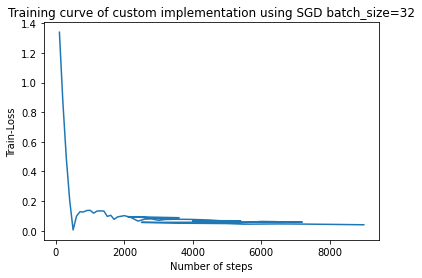
\includegraphics[width=8cm]{images/q3.2-custom.png}
        \caption{} \label{fig:part2}
	\end{figure}
    \end{soln}
    \item Implement the same network in PyTorch (or any other framework). You can use all the features of the framework e.g. auto-grad etc. Evaluate it on MNIST dataset, report test errors, and learning curve. (2 pts)

        \begin{soln}
        I implemented the same model fully on PyTorch, making use of the nn.Module class and AutoGrad. The accuracy was slightly lower,91.58\%, than my implementation(I checked the code multiple times). I believe the difference could be due to how Pytorch implements cross-entropy loss(logits instead of softmax as input) and updates gradients. I didn't tune the hyperparameters of this model further, as the purpose of this question was to implement the same model as in Part 2. The training curve can be found in \ref{fig:part3}.
        \begin{figure}[hbt!]
		\centering
		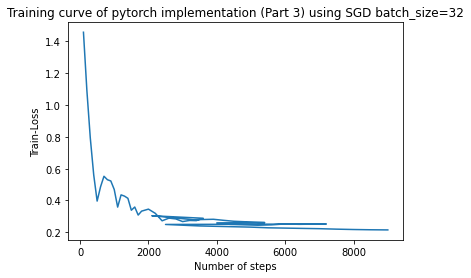
\includegraphics[width=8cm]{images/q3.3-pytorch.png}
        \caption{} \label{fig:part3}
	\end{figure}
    \end{soln}
    \item Try different weight initialization a) all weights initialized to 0, and b) initialize the weights randomly between -1 and 1. Report test error and learning curves for both. (You can use either of the implementations) (3 pts)\\
    \begin{soln}
        Since my implementation gave better accuracy, I proceeded with my implementation of the model for this question. The zero-initialization case gave a very bad accuracy and random initialization case gave a comparable value to my original implementation. The training curves can be found in \ref{fig:part4a} and \ref{fig:part4b}. The test accuracies were 11.35\% and 94.46\%, respectively, for (a) and (b). This shows the importance of initialization. Zero-initialization gives poor accuracy, and smaller weights are better(my original initialization was in $[-0.07,0.07]$ ).

        \begin{figure}[hbt!]
		\centering
		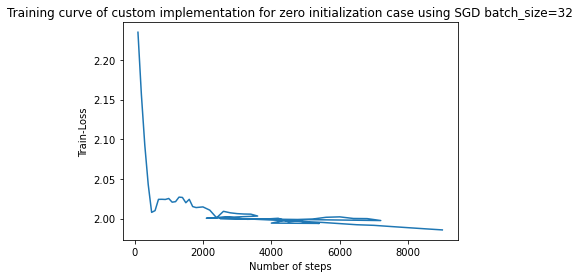
\includegraphics[width=8cm]{images/q3.4(a)-zero_init.png}
        \caption{} \label{fig:part4a}
	\end{figure}

 \begin{figure}[hbt!]
		\centering
		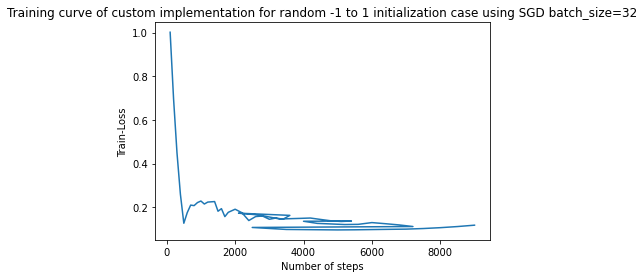
\includegraphics[width=8cm]{images/q3.4(b)-random_init.png}
        \caption{} \label{fig:part4b}
	\end{figure}
        
    \end{soln}
\end{enumerate}

You should play with different hyperparameters like learning rate, batch size, etc. for your own learning. You only need to report results for any particular setting of hyperparameters. You should mention the values of those along with the results. Use $d_1 = 300$, $d_2 = 200$, $d_3 = 100$. For optimization use SGD (Stochastic gradient descent) without momentum, with some batch size say 32, 64, etc. MNIST can be obtained from here (https://pytorch.org/vision/ stable/datasets.html)

\bibliographystyle{apalike}
\end{document}
